\section{Aviation context in Indonesia}
\paragraph{} Indonesia is the fourth most populated country in the world and the largest economy in south-east Asia. Indonesia is also, a growing touristic destination because its outstanding nature marvels and cultural monuments. It’s topography which is composed by many island makes essential the domestic air transport.

Jakarta (located at the island of Java) is the centre of government, commerce and industry of Indonesia. Currently Jakarta has an international airport (Soekarno-Hatta International Airport). It operates around the 250\% over its design capacity and an interesting fact is that last year 40\% of its flights were delayed. Efforts have been made to decrease this problem opening a small military airport for civilian domestic flights. Nevertheless, the problem still persists. 

The current Jakarta airport cannot be expanded, due to nearby neighbourhoods. "Some news have been recently published by Jakarta authorities confirming the urge of a new airport around Jakarta to absorb the saturated traffic of the Soekarno-Hatta International Airport, even after constructing a new runway and terminal on it. 

All in all, it is essential to construct a new airport. Moreover, the secondary airport, really small, is only focused on military and private services and does not have enough fields at its surroundings to expand, as Jakarta air traffic requires. 

Therefore, the need for a new commercial airport near Jakarta is clear. Coming up next, a project for this new airport will be developed.

\clearpage

	\subsection{Airport location}
\paragraph{}The main idea to find a good location was to put the new Jakarta airport in an area not too far from the city with enough space to build a big airport which has opportunities to expand in a further future.

Following this parameters, the location chosen geographically is situated to the east of the city of Jakarta at 32 km from the city center. It is also located above the emerging city of Bekasi that in the last years is increasing its industry hosting several multinationals. In addition, the terrain is not edified yet and extensive, plus it is non-mountainous and obstacles-free.

\begin{figure}[H]
	\centering
	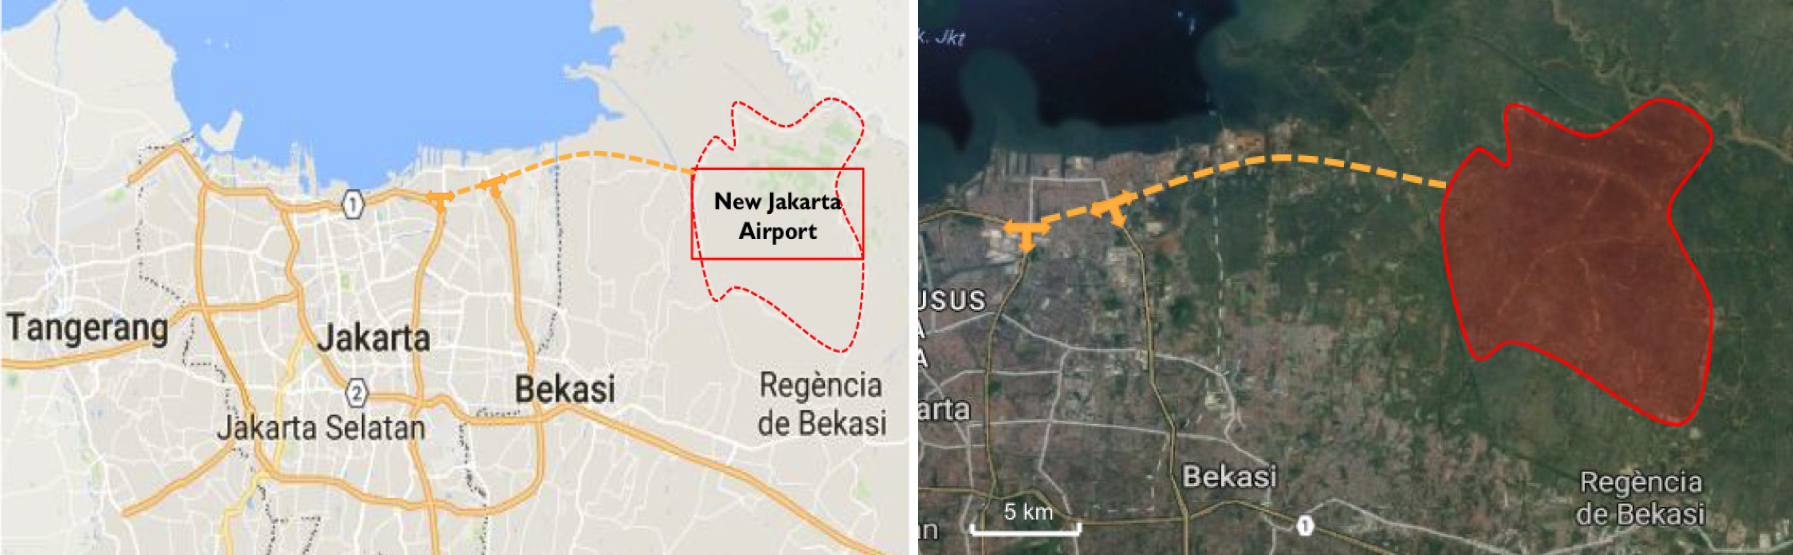
\includegraphics[clip, trim=0cm 0cm 0cm 0cm, width=1\textwidth]{./images/PROGNOSIS/airport_location}
	\caption{Bekasi-East Jakarta Airport selected location.}
	\label{airprt-location}
\end{figure}

It is a huge free obstacle flat field, without relevant slope gradients and the terrain is not edified yet. It is an exceptional location due to its huge amount of terrain available where companies could settle down taking advantage of the airport proximity, low terrain costs and direct connection with the down town. There is enough space to become also a logistic distribution centre of the island and Indonesia.

Finally, as it is an almost virgin land, communication is limited. Therefore, the solution is easy. The present Jakarta motorway will be extended. As it is shown on Fig. \ref{airprt-location} indicated with a discontinuous line, there will be two connections between the current and the new highway. 

Connection between airports will be achieved thanks to this new built highway. It will take 40min from door to door. Connection network of free-busses between both airports will make transfers safe and easy. There will be also available buses to and from the city centre, at low prices. During rush hours, a specific way will be delimited only for airport bus transfers. 

	
	\subsection{Current traffic}
\paragraph{} The starting point has been Soekarno-Hatta Airport. As it can be seen on fig.\ref{paxYears}, currently Soekarno-Hatta Airport is handling volumes of passengers around 50 million passengers by year.

\begin{figure}[H]
	\centering
	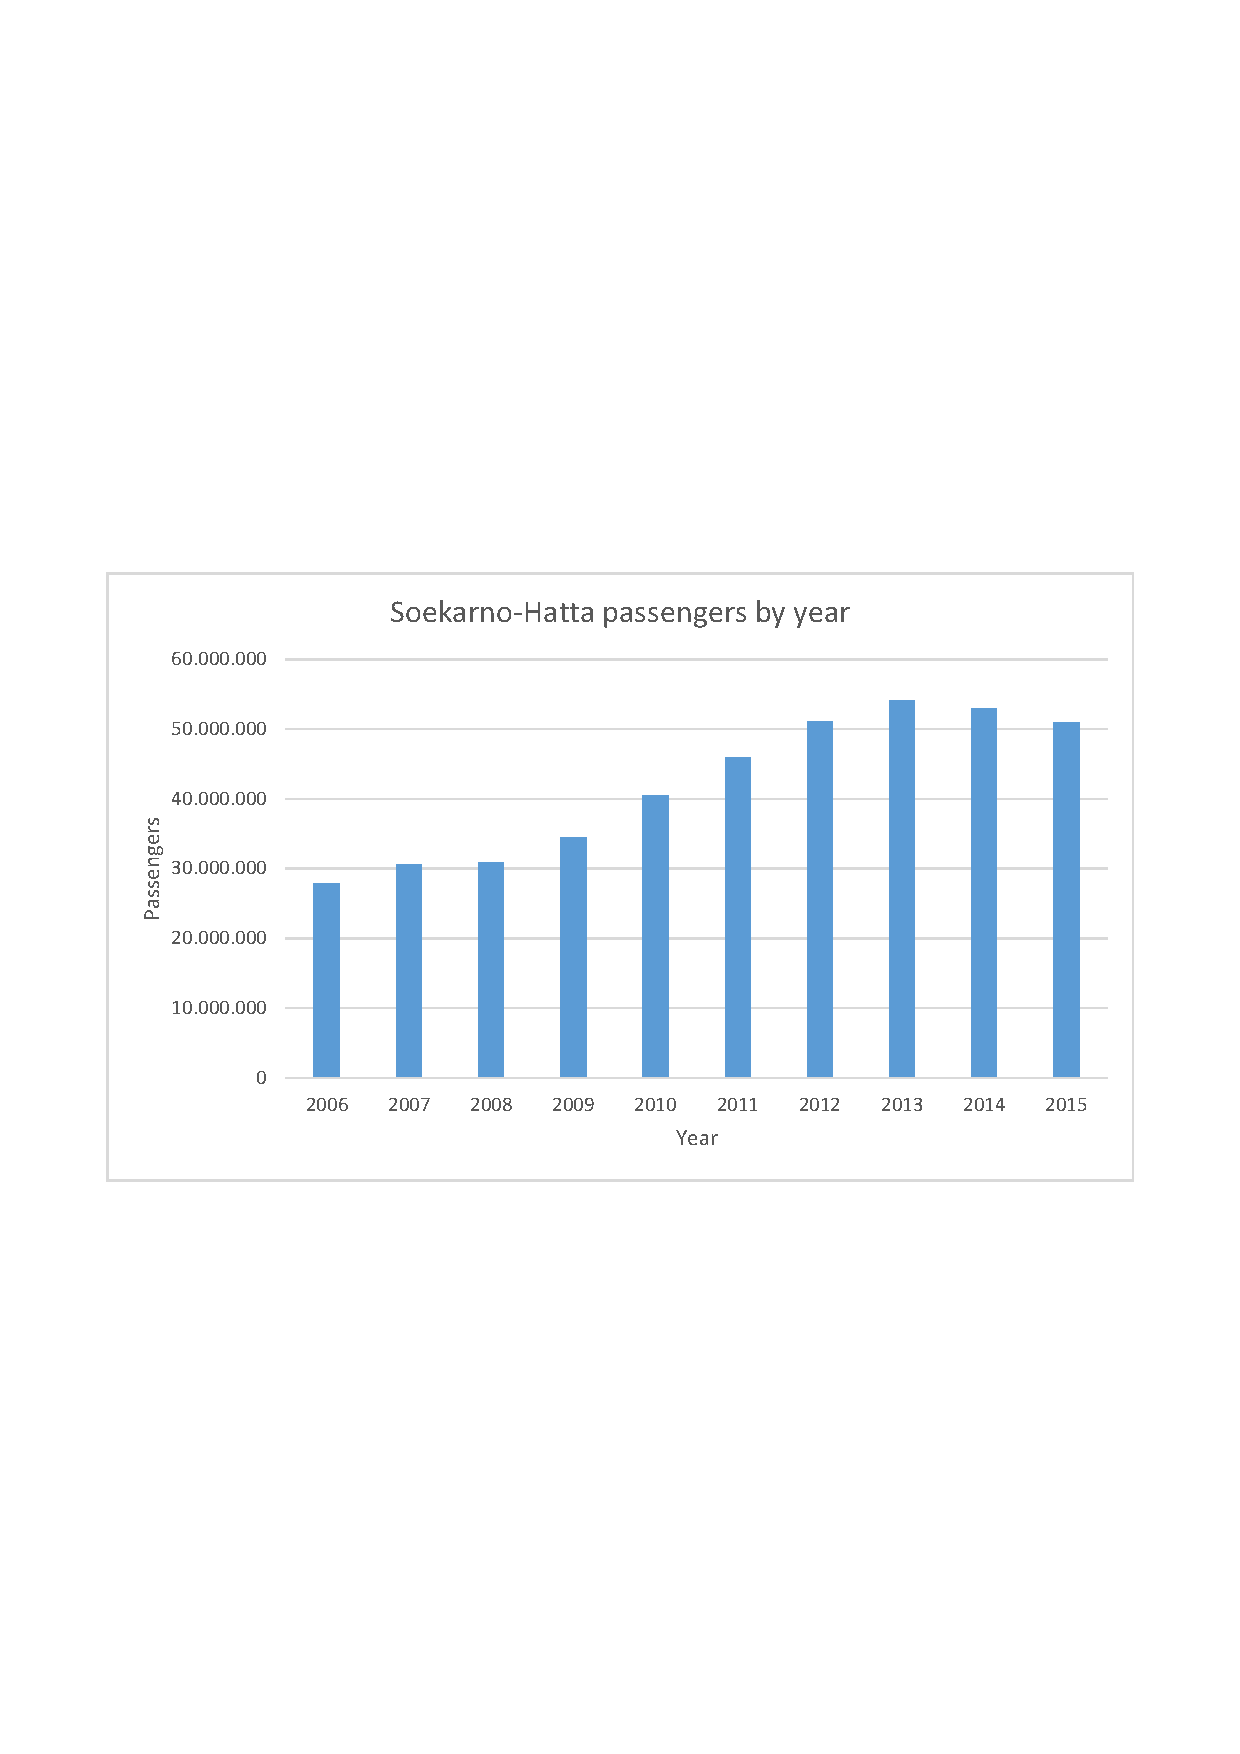
\includegraphics[clip, trim=2cm 10cm 2cm 10cm, width=1\textwidth]{./images/PROGNOSIS/paxYears}
	\caption{Soekarno-Hatta International Airport passengers by years }
	\label{paxYears}
\end{figure}	

Operations on a mean day have the following pattern:
\begin{figure}[H]
	\centering
	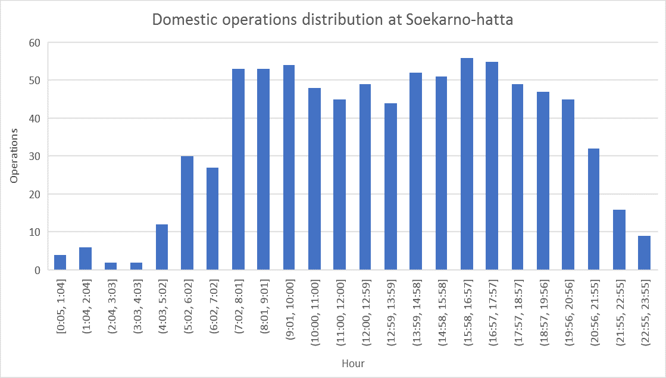
\includegraphics[clip, trim=0.1cm 0.1cm 0.1cm 0.1cm, width=0.8\textwidth]{./images/PROGNOSIS/hourDom}
	\caption{Soekarno-Hatta International Airport domestic flights distribution on busy day.}
	\label{hourDom}
\end{figure}

	
%\begin{figure}[H]
%	\centering
%	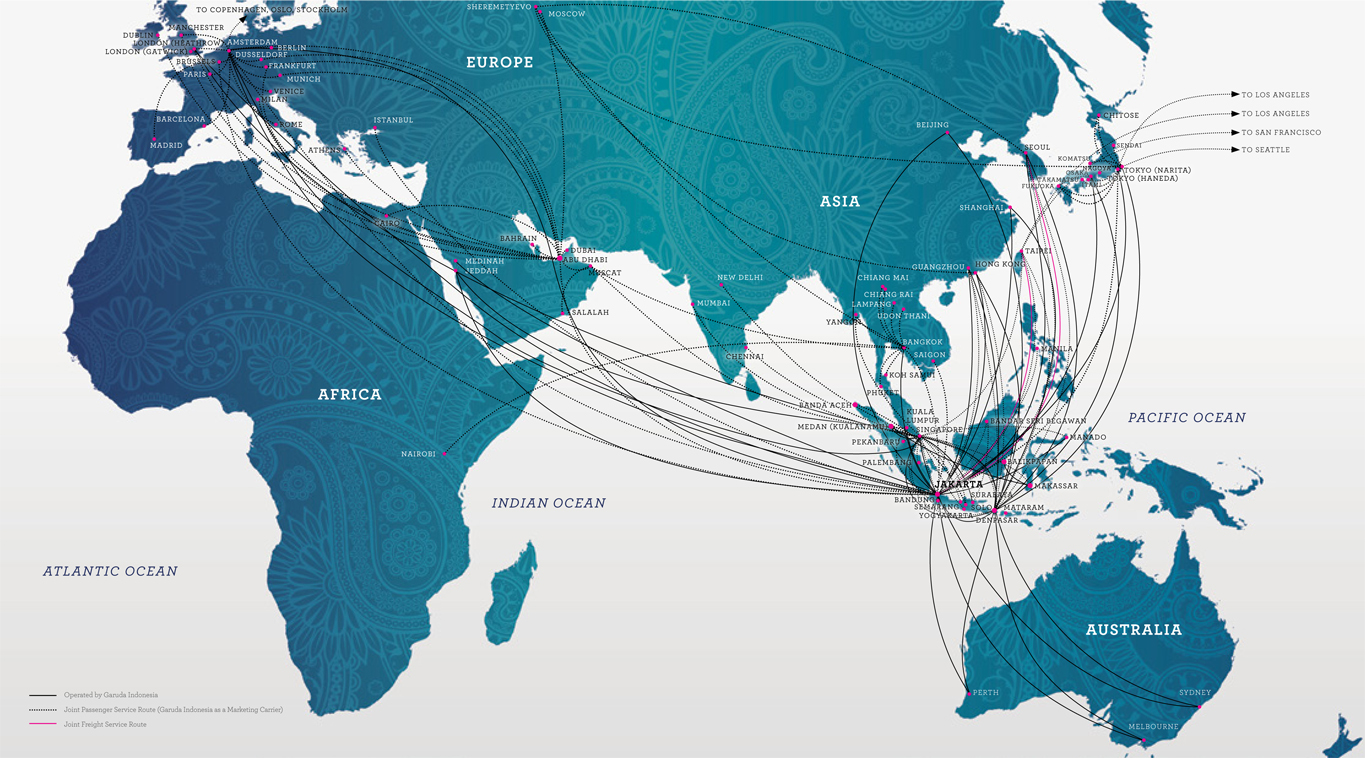
\includegraphics[clip, trim=0cm 0cm 0cm 0cm, width=1\textwidth]{./images/PROGNOSIS/international-routes}
%	\caption{Soekarno-Hatta International Airport routes }
%	\label{Soekarno-routes}
%\end{figure}
	\subsection{Occupation factor}
	\paragraph{} Occupation factor will be 77\%
	https://www.iata.org/whatwedo/workgroups/Documents/MCTF/AMC-Exec-Comment-FY14.pdf
	\cite{IATA_PLF}x
	
	